In chapter~\ref{ch:mvica1} and chapter~\ref{ch:mvica2}, we have introduced MultiView ICA, a well principled method to perform shared response modeling. 
While MultiView ICA yields good practical results, it does not model subject specific deviations from the shared
response. Yet, the magnitude of the response may differ across subjects \cite{penny2007random}, as does any noise due to heart beats, respiratory artefacts or head movement~\cite{liu2016noise}.
%

This drawback is shared by most GroupICA methods that often rely on single
subject ICA to recover the shared response. In addition, such methods are typically unable to separate Gaussian components.

In contrast, the framework of Independent vector analysis
(IVA)~\cite{lee2008independent, anderson2011joint} allows subject specific
variability in the unmixed data. However, the two most common implementations (IVA-L~\cite{lee2008independent} and IVA-G~\cite{anderson2011joint}) only estimate view-specific components, and do not model or extract a shared response. 
They are thus not well-suited for modelling the dependencies between views in
functional brain imaging, as we will argue in detail below.

In this chapter, we introduce Shared ICA (ShICA), where each dataset is modeled as a linear transform of shared independent components contaminated by additive Gaussian noise. ShICA allows for principled extraction of the shared components (or responses) in addition to view-specific components. 
%
Since it incorporates a statistically sound noise model, it enables optimal inference (minimum mean squared error, MMSE) of the shared responses.

We first analyse the theoretical properties of the ShICA model, before providing powerful inference algorithms.
First, we exhibit necessary and sufficient conditions for ShICA to be identifiable (previous work only shows local identifiability~\cite{anderson2014independent}), in the presence of Gaussian or non-Gaussian components. 
%
We then introduce an algorithm called ShICA-J that uses Multiset CCA to fit the model when all the components are assumed to be Gaussian. We exhibit necessary and sufficient conditions for Multiset CCA to be able to fit the model (previous work only gives sufficient conditions~\cite{li2009joint}) and provide examples on which ShICA-J can recover the mixing matrices, while Multiset CCA cannot. 
%
We next point out a practical problem, namely that even a small sampling noise can lead to large rotations of unmixing matrices when Multiset CCA is used. To address this issue and recover the correct unmixing matrices, we propose to apply joint diagonalization to the result of Multiset CCA.
%
We further introduce ShICA-ML, a maximum likelihood estimator of ShICA that models non-Gaussian components using a Gaussian mixture model. 
%
While ShICA-ML yields more accurate components, ShICA-J is significantly faster and offers a great initialization to ShICA-ML.

\section{Shared ICA (ShICA): an identifiable multi-view model}
We assume a similar generative model as in MultiViewICA:
\begin{equation}
  \label{eq:model}
   \xb_i = A_i(\sbb + \nb_i)
\end{equation}

Like in MultiView ICA we assume that the shared components are statistically independent $p(\sbb) = \prod_{j=1}^p p(s_j)$, and
that the individual noises are Gaussian and independent from the shared
components. We assume $\nb_i \sim\mathcal{N}(0, \Sigma_i)$, where the matrices
$\Sigma_i$ are assumed diagonal and positive. This contrasts with MultiView ICA: the individual noise variances are learned and are not assumed to be the same across
components or subjects.
We further assume that there are at least 3 views: $m \geq 3$. 

In contrast to almost all existing works, we assume that some components (possibly all of them) may be Gaussian, and denote $\mathcal{G}$ the set of Gaussian components: $\sbb_j \sim \mathcal{N}(0, 1)$ for $j \in \mathcal{G}$. The other components are non-Gaussian: for $j\notin \mathcal{G}$, $\sbb_j$ is non-Gaussian.


\paragraph{Identifiability} The parameters of the model are $\Theta = (A_1, \dots, A_m, \Sigma_1, \dots, \Sigma_m)$. We are interested in the identifiability of this model: given observations $\xb_1,\dots, \xb_m$ generated with parameters $\Theta$, are there some other $\Theta'$ that can generate the same observations?
Let us consider the following assumption that requires that the individual noises for Gaussian components are sufficiently diverse:
%
\begin{assumption}[Noise diversity in Gaussian components]
\label{ass:diversity}
For all $j, j' \in \mathcal{G}, j \neq j'$, the sequences $(\Sigma_{ij})_{i=1 \dots m}$ and $(\Sigma_{ij'})_{i=1 \dots m}$ are different where $\Sigma_{ij}$ is the $j, j$ entry of $\Sigma_i$
\end{assumption}

It is readily seen that there is one trivial set of indeterminacies in the problem: if $P \in \mathbb{R}^{p \times p}$ is a sign and permutation matrix the parameters $(A_1 P, \dots, A_m P, P^{\top}\Sigma_1 P, \dots, P^{\top} \Sigma_m P)$ also generate $\xb_1,\dots, \xb_m$. The following theorem shows that under the above assumption, these are the only indeterminacies of the problem.

\begin{theorem}[Identifiability]
\label{thm:identif}
We suppose Assumption~\ref{ass:diversity}. We let $\Theta'=(A_1', \dots, A_m', \Sigma_1', \dots,\Sigma_m')$ another set of parameters, and assume that they also generate $\xb_1,\dots, \xb_m$. Then, there exists a sign and permutation matrix $P$ such that for all $i$, $A_i'=A_iP$, and $\Sigma_i'= P^{\top} \Sigma_i P$.
\end{theorem}
\label{proof:identif}
\begin{proof}
By hypothesis, the covariances verify $C_{ij} =\bbE[\xb_i\xb_j^\top] = A_i(I_p + \delta_{ij}\Sigma_i)A_j^{\top} = A'_i(I_p + \delta_{ij}\Sigma'_i){A'_j}^{\top}$ for all $i, j$. We let $P_i=A_i^{-1}A_i'$. The previous relationship for $j\neq i$ gives $P_iP_j^{\top} = I_p$. Because there are more than 3 views, there is another integer $k \notin\{i,j\}$, and we have $P_iP_k^{\top}= P_jP_k^{\top}=I_p$. This shows that $P_i = P_j$: all these matrices are equal, and we call $P$ their common value. The previous equation also gives $PP^{\top} = I_p$, so $P$ is orthogonal. 
%
We have that $s + n_i$ and $s' + n_i'$ have independent components and $s + n^i
= P(s' + n_i')$. Lemma~\ref{lemma:ica} in appendix~\ref{app:sec:lemmas} (a direct consequence of classical ICA results~\cite{comon1994independent}, Theorem 10) gives $P=\Pi^{-1} \Omega \Pi'$ where $\Pi$ and $\Pi'$ are sign and permutation matrices such that the first $g$ components of $\Pi(s + n_i)$ and $\Pi'(s' + n_i')$ are Gaussian, and $\Omega$ is a block diagonal matrix given by
\[
\Omega = \begin{bmatrix} \Omega_g & 0 \\ 0 & I_{p - g} \end{bmatrix}
\]
where $\Omega_g$ is orthogonal.
%
We call $A^{(g)}$ the first $g \times g$ block of a matrix $A$ so that $\Omega^{(g)} = \Omega_g$.

Then, considering only the Gaussian components, we can write for $i=j$:  
$(\Pi \Sigma_i)^{(g)} = \Omega_g (\Pi' \Sigma'_i)^{(g)} \Omega_g^{\top}$ for all
$i$. This, combined with Assumption~\ref{ass:diversity}, implies that $\Omega_g$
is a sign and permutation matrix (see Lemma~\ref{lemma:eigdecomp} in appendix~\ref{app:sec:lemmas}) and therefore $P$ is a sign and permutation matrix. Then it follows that $I + \Sigma_i = P(I + \Sigma'_i)P^{\top}$ and therefore $\Sigma_i = P \Sigma'_i P^{\top}$ so $\Sigma'_i = P^{\top} \Sigma_i P$.
\end{proof}

Identifiability in the Gaussian case is a consequence of the identifiability results in~\cite{via2011joint} and in the general case, local identifiability results can be derived from the work of ~\cite{anderson2014independent}. 
%
However local identifiability only shows that for a given set of parameters there exists a neighborhood in which no other set of parameters can generate the same observations~\cite{rothenberg1971identification}. In contrast, the proof of Theorem~\ref{thm:identif} shows global identifiability.

% \pierre{Lacks biblio: this result is not from us per se}
Theorem~\ref{thm:identif} shows that the task of recovering the parameters from
the observations is a well-posed problem, under the sufficient condition of
Assumption~\ref{ass:diversity}.  We also note that
Assumption~\ref{ass:diversity} is necessary for identifiability. For instance,
if $j$ and $j'$ are two Gaussian components such that $\Sigma_{ij} =
\Sigma_{ij'}$ for all $i$, then a global rotation of the components $j, j'$
yields the same covariance matrices. The current work assumes $m \geq 3$. In appendix~\ref{app:identifiability} we give an identifiability result for $m=2$.



\section{Estimation of components with noise diversity via joint-diagonalization}

We now consider the computational problem of efficient parameter inference. This section considers components with noise diversity, while the next section deals with non-Gaussian components.


\subsection{Fitting ShICA via Multiset CCA}
If we assume that the components are all Gaussian, % \aapo{[Aapo: move to section 3.1?]}
the covariance of the observations given by
$C_{ij}=  \bbE[\xb_i\xb_j^\top] = A_i(I_p + \delta_{ij}\Sigma_i)A_j^{\top}\enspace
$ are sufficient statistics and methods using only second order information, like Multiset CCA, are candidates to estimate the parameters of the model.
Consider the
matrix $C \in \bbR^{pm \times pm}$ containing $m \times m$ blocks of size $p
\times p$
such that the block $i,j$ is given by $C_{ij}$. Consider the matrix $D$ identical to $C$ excepts that the non-diagonal blocks are filled with zeros. 
Generalized CCA consists in the following generalized eigenvalue problem:
\begin{equation}
\label{eq:eigv}
    C \ub = \lambda D\ub,\enspace \lambda > 0,\enspace \ub\in\bbR^{pm} \enspace .
\end{equation}
  
Consider the matrix $U = [\ub^1, \dots, \ub^p] \in \mathbb{R}^{mp \times p}$ formed by concatenating the $p$ leading eigenvectors of the previous problem ranked in decreasing eigenvalue order. Then, consider $U$ to be formed of $m$ blocks of size $p \times p$ stacked vertically and define $(W_i)^{\top}$ to be the $i$-th block. These $m$ matrices are the output of Multiset CCA. We also denote $\lambda_1 \geq \dots \geq \lambda_p$ the $p$ leading eigenvalues of the problem.
  %\aapo{[Very difficultto understand! First define the matrix by u's, and then say that you take blocks out of it to define the W.]}

An application of the results of \cite{li2009joint} shows that Multiset CCA recovers the mixing matrices of ShICA under some assumptions.
%
\begin{proposition}[Sufficient condition for solving ShICA via Multiset CCA~\cite{li2009joint}]
Let $r_{ijk} = (1 + \Sigma_{ik})^{-\frac12} (1 + \Sigma_{jk})^{-\frac12}$.
%\bt{Hm. What is $\Sigma_{ik}$ ?}
Assume that $(r_{ijk})_k$ is non-increasing. Assume that the maximum eigenvalue $\nu_k$ of matrix $R^{(k)}$ of general element $(r_{ijk})_{ij}$ is such that  $\nu_k = \lambda_k$ 
%\bt{$\nu_k$ is not defined}
.
Assume that $\lambda_1 \dots \lambda_p$ are distinct.
Then, there exists scale matrices $\Gamma_i$ such that $W_i = 
\Gamma_i A_i^{-1}$ for all $i$.
\end{proposition}
This proposition gives a sufficient condition for solving ShICA with Multiset CCA. It needs a particular structure for the noise covariances as well as specific ordering for the eigenvalues. The next theorem shows that we only need $\lambda_1 \dots \lambda_p$ to be distinct for Multiset CCA to solve ShICA:
\begin{assumption}[Unique eigenvectors]
  \label{ass:uniqueeig}
$\lambda_1 \dots \lambda_p$ are distinct.
\end{assumption}
% \pierre{talk a bit about these assumptions and the eigenvalue distribution}
\begin{theorem}
  \label{th:eig}
  We suppose
  Assumption~\ref{ass:uniqueeig} (only). Then, there exists a permutation matrix $P$ and scale matrices $\Gamma_i$ such that $W_i = P\Gamma_i A_i^{-1}$ for all $i$.
\end{theorem}
\label{proof:eig}
\begin{proof}
  Let us denote $W \in \bbR^{mp \times mp}$ the block diagonal matrix with block $i$ given by
  $(A_i)^{-1}$. We have $C \ub = \lambda D \ub  \iff W C W^\top \zb = \lambda W D W^\top \zb
  $ where $\ub = W^\top \zb$. We call $\zb$ a reduced eigenvector.
  Each
  block in $W C W^\top$ and in $W D W^\top$ is diagonal so any reduced eigenvector $\zb = \begin{bmatrix} \zb_1 \\ \vdots \\ \zb_m \end{bmatrix}$ is
  such that the matrix $Z = [\zb_1 \dots \zb_m]$ has exactly one non-zero line.
  Following Lemma~\ref{lemma:nonzerocoord} in appendix~\ref{app:sec:lemmas}, the first $p$ leading reduced
  eigenvectors $\zb^1, \dots, \zb^p$ all have different first non-zero coordinates.
  Therefore the concatenation of the first $p$ leading reduced eigenvectors is given
  by $[\zb^1, \dots \zb^p] = \begin{bmatrix} \Gamma_1 \\ \vdots \\ \Gamma_m \end{bmatrix} P^{\top}$ where $P^{\top} \in \mathbb{R}^{p \times p}$ is a permutation matrix and $\Gamma_i
  \in \mathbb{R}^{p \times p}$ is a diagonal matrix. Therefore, the first $p$
  eigenvectors are given by $[\ub^1 \dots \ub^p] = \begin{bmatrix} W_1^{\top} \\ \vdots \\ W_m^{\top} \end{bmatrix} = \begin{bmatrix} (A_1^{-1})^{\top} \Gamma_1 P^{\top} \\ \vdots \\ (A_m^{-1})^{\top} \Gamma_m P^{\top} \end{bmatrix}$  and so $W_i = P \Gamma_i A_i^{-1}$
\end{proof}

This theorem means that solving the generalized eigenvalue problem~\eqref{eq:eigv} allows to recover the mixing matrices up to a scaling and permutation: this form of generalized CCA recovers the parameters of the statistical model.
Note that Assumption~\ref{ass:uniqueeig} is also a necessary condition. Indeed, if two eigenvalues are identical, the eigenvalue problem is not uniquely determined.

%\aapo{[Aapo: due to lack of space the rest of this subsection could be moved to suppl material.]}
We have two different Assumptions, \ref{ass:diversity} and \ref{ass:uniqueeig}, the first of which guarantees theoretical identifiability as per Theorem~\ref{thm:identif} and the second guarantees consistent estimation by Multiset CCA as per Theorem~\ref{th:eig}. Next we will discuss their connections, and show some limitations of the Multiset CCA approach. To begin with, we have the following result about the eigenvalues of the problem~\eqref{eq:eigv} and the $\Sigma_{ij}$.
% \pierre{best not to use a pointer to the appendix in the text, just state the following result}
\begin{prop}
  \label{prop:eigvals_from_noise}
  For $j\leq p$, let $\lambda_j$ the largest solution of $ \sum_{i=1}^m\frac{1}{\lambda_j(1 + \Sigma_{ij}) -\Sigma_{ij}}=1$. Then, $\lambda_1, \dots, \lambda_p$ are the $p$ largest eigenvalues of problem~\eqref{eq:eigv}.
\end{prop}
It is easy to see that we then have $\lambda_1, \dots, \lambda_p$ greater than $1$, while the remaining eigenvalues are lower than $1$.
From this proposition, two things appear clearly. First, Assumption~\ref{ass:uniqueeig} implies Assumption~\ref{ass:diversity}.
%
Indeed, if the $\lambda_j$'s are distinct, then the sequences $(\Sigma_{ij})_i$ must also be different from the previous proposition.
%
This is expected as from Theorem~\ref{th:eig}, Assumption~\ref{ass:uniqueeig} implies identifiability, which in turn implies Assumption~\ref{ass:diversity}.
% \pierre{I wrote this but this is really pompous}

Prop.~\ref{prop:eigvals_from_noise} also allows us to derive cases where Assumption~\ref{ass:diversity} holds but not Assumption~\ref{ass:uniqueeig}. The following Proposition shows that we can chose parameters of the model so that the model is identifiable but it cannot be solved using Multiset CCA:
\begin{prop}
\label{counter}
Assume that for two integers $j, j'$, the sequence $(\Sigma_{ij})_i$ is a permutation of $(\Sigma_{ij'})_i$, i.e. that there exists a permutation of $\{1,\dots, p\}$, $\pi$, such that for all $i$, $\Sigma_{ij} = \Sigma_{\pi(i)j'}$.  Then, $\lambda_j = \lambda_{j'}$.
\end{prop}
In this setting, Assumption~\ref{ass:diversity} holds so ShICA is identifiable, while Assumption~\ref{ass:uniqueeig} does not hold, so Multiset CCA cannot recover the unmixing matrices.




\subsection{Sampling noise and improved estimation by joint diagonalization} \label{sec:samplingnoise}


The consistency theory for Multiset CCA developed above is conducted under the assumption that the
covariances $C_{ij}$ are the true covariances of the model, and not
approximations obtained from observed samples. In practice, however, a serious limitation of Multiset CCA is that even a slight error of estimation on the covariances, due to ``sampling noise'', can yield a large error in the estimation of the unmixing matrices, as will be shown next.


\begin{wrapfigure}{r}{.4\textwidth}
\centering
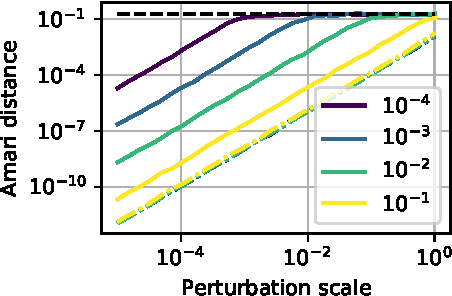
\includegraphics[width=.99\linewidth]{figures/amvica/multicca_gap_jd.pdf}
\caption{Amari distance between true mixing matrices and estimates of Multiset CCA when covariances are perturbed. Different curves correspond to different eigen-gaps. When the gap is small, a small perturbation can lead to complete mixing. Joint-diagonalization (colored dotted lines) fixes the problem.}
\label{fig:cca_gap}
\end{wrapfigure}
We begin with an empirical illustration. We take $m=3$, $p=2$, and $\Sigma_i$ such that $\lambda_1 = 2 + \varepsilon$ and $\lambda_2 =2$ for $\varepsilon > 0$.
%
In this way, we can control the \emph{eigen-gap} of the problem, $\varepsilon$.
%
%
We take $W_i$ the outputs of Multiset CCA applied to the true covariances $C_{ij}$.
%
Then, we generate a perturbation $\Delta = \delta \cdot S$, where $S$ is a random positive symmetric $pm \times pm$ matrix of norm $1$, and $\delta >0$ controls the scale of the perturbation. 
%
We take $\Delta_{ij}$ the $p\times p$ block of $\Delta$ in position $(i, j)$, and $\tilde{W}_i$ the output of Multiset CCA applied to the covariances $C_{ij} + \Delta_{ij}$.
%
We finally compute the sum of the Amari distance between the $W_i$ and $\tilde{W}_i$: the Amari distance measures how close the two matrices are, up to scale and permutation~\cite{amari1996new}.
%\Alex{add ref to paper that explicits the Amari distance}
Fig~\ref{fig:cca_gap} displays the median Amari distance over 100 random repetitions, as the perturbation scale $\delta$ increases. The different curves correspond to different values of the eigen-gap $\varepsilon$. We see clearly that the robustness of Multiset CCA critically depends on the eigen-gap, and when it is small, even a small perturbation of the input (due, for instance, to sampling noise) can lead to large estimation errors.


This problem is very general and well studied~\cite{stewart1973error}: the mapping from matrices to (generalized) eigenvectors is highly non-smooth.
%
However, the gist of our method is that the \emph{span} of the leading $p$ eigenvectors is smooth, as long as there is a large enough gap between  $\lambda_p$ and $\lambda_{p+1}$.
For our specific problem we have the following bounds, derived from Prop.~\ref{prop:eigvals_from_noise}.
\begin{prop}
  We let $\sigma_{\max} = \max_{ij}\Sigma_{ij}$ and $\sigma_{\min} = \min_{ij}\Sigma_{ij}$. Then, $\lambda_p \geq 1 + \frac{m-1}{1+\sigma_{\max}}$, while $\lambda_{p+1}\leq 1 - \frac{1}{1 + \sigma_{min}}$.
\end{prop}
As a consequence, we have $\lambda_{p} -\lambda_{p+1} \geq \frac{m-1}{1+\sigma_{\max}} + \frac{1}{1+ \sigma_{\min}}$: the gap between these eigenvalues increases with $m$, and decreases with the noise power.

  \begin{algorithm}[H]
    \SetAlgoLined
  \caption{ShICA-J}
  \label{algo:shicaj}
  \KwIn{Covariances $\tilde{C}_{ij} =
    \bbE[\xb_i\xb_j^{\top}]$}
    $(\tilde{W}_i)_i \leftarrow \mathrm{MultisetCCA}((\tilde{C}_{ij})_{ij})$ \\
        $Q \leftarrow
        \mathrm{JointDiag}((\tilde{W}_i\tilde{C}_{ii}\tilde{W}_i^{\top})_i)$ \\
       $\Gamma_{ij} \leftarrow Q\tilde{W}_i\tilde{C}_{ij}W_j^\top Q^\top$ \\
       $(\Phi_i)_i \leftarrow \mathrm{Scaling}((\Gamma_{ij})_{ij})$ \\
   \Return{Unmixing matrices $(\Phi_iQ\tilde{W}_i)_i$}
  \end{algorithm}

In this setting, when the magnitude of the perturbation $\Delta$ is smaller than $\lambda_{p}-\lambda_{p+1}$, ~\cite{stewart1973error} indicates that $\mathrm{Span}([W_1, \dots, W_m]^{\top})\simeq \mathrm{Span}([\tilde{W}_1,\dots, \tilde{W}_m]^\top)$, where $[W_1, \dots, W_m]^{\top}\in\bbR^{pm\times p}$ is the vertical concatenation of the $W_i$'s.
In turn, this shows that there exists a matrix $Q\in\bbR^{p\times p}$ such that
%
%
\begin{equation}
    \label{eq:justif_jd}
    W_i \simeq Q\tilde{W}_i\enspace \text{for all} \enspace i.
\end{equation}

We propose to use joint-diagonalization to recover the matrix $Q$. Given the $\tilde{W}_i$'s, we consider the set of symmetric matrices $\tilde{K}_i = \tilde{W}_i\tilde{C}_{ii}\tilde{W}_i^{\top}$, where $\tilde{C}_{ii}$ is the contaminated covariance of $\xb_i$. Following Eq.~\eqref{eq:justif_jd}, we have $Q\tilde{K}_iQ^{\top} = W_i \tilde{C}_{ii}W_i^{\top}$, and using Theorem~\ref{th:eig}, we have $Q\tilde{K}_iQ^{\top} = P\Gamma_i A_i^{-1}\tilde{C}_{ii}A_i^{-\top}\Gamma_iP^{\top}$. Since $\tilde{C}_{ii}$ is close to $C_{ii} = A_i (I_p + \Sigma_i)A_i^\top$, the matrix $P\Gamma_i A_i^{-1}\tilde{C}_{ii}A_i^{-\top}\Gamma_iP^{\top}$ is almost diagonal.
%
In other words, the matrix $Q$ is an approximate diagonalizer of the $\tilde{K}_i$'s, and we approximate $Q$ by joint-diagonalization of the $\tilde{K}_i$'s. In Fig~\ref{fig:cca_gap}, we see that this procedure mitigates the problems of multiset-CCA, and gets uniformly better performance regardless of the eigen-gap.
%
In practice, we use a fast joint-diagonalization
algorithm~\cite{ablin2018beyond} to minimize a joint-diagonalization criterion
for positive symmetric matrices~\cite{pham2001joint}. The estimated unmixing
matrices
\begin{align}
U_i = Q\tilde{W}_i
\end{align}
correspond to the true unmixing matrices only up to some scaling: the information that the components are of unit variance is lost.

\textbf{Scale estimation}
We form the matrices $\Gamma_{ij} = U_i\tilde{C}_{ij}U_j^\top$. In order to
estimate the scalings, we solve
\begin{align}
\loss_{\Phi} = \min_{(\Phi_i)} \sum_{i\neq j} \| \Phi_i \diag(\Gamma_{ij}) \Phi_j - I_p \|_F^2
\end{align}
where the $\Phi_i$ are diagonal matrices.
The gradient is given by
\begin{align}
  \partialfrac{\Phi_i}{\loss_{\Phi}} = 2\sum_{j \neq i} (\Phi_i \diag(Y_{ij}) \Phi_j - I_p) \Phi_j
\end{align}
Therefore we get
\begin{align}
  &\partialfrac{\Phi_i}{\loss_{\Phi}} = 0 \\
  &\iff 2\sum_{j \neq i} (\Phi_i \diag(Y_{ij}) \Phi_j - I_p) \Phi_j = 0 \\
  &\iff \Phi_i \sum_{j \neq i} \diag(Y_{ij}) \Phi_j^2 - \sum_{j \neq i} \Phi_j = 0 \\
  &\iff \Phi_i = \frac{\sum_{j \neq i} \Phi_j}{\sum_{j \neq i} \diag(Y_{ij}) \Phi_j^2}
    \label{eq:phiupdates}
\end{align}
We then iterate formula~\eqref{eq:phiupdates} over $i$ until convergence.
The final estimates of the unmixing matrices are given by
\begin{align}
  (\Phi_i U_i)_{i=1}^m
\end{align}
The full procedure, called ShICA-J, is summarized in Algorithm~\ref{algo:shicaj}.

\subsection{Estimation of noise covariance and inference of shared components}

In practice, it is important to estimate noise co-variances $\Sigma_i$ in order to take advantage of the fact that some views are noisier than others. As it is well known in classical factor analysis, modelling noise variances allows the model to virtually discard variables, or subjects, that are particularly noisy. 

Using the ShICA model with Gaussian components, we derive noise covariances estimate directly from maximum likelihood. We use an expectation-maximization (EM) algorithm, which is especially fast because noise updates are in closed-form. Following derivations given in appendix~\ref{conditional_density}, the sufficient statistics in the E-step are given by 
\begin{align}
\label{mmse1}
&\EE[\sbb|\xb]= \left(\sum_{i=1}^m \Sigma_i^{-1}  + I \right)^{-1}  \sum_{i=1}^m \left(\Sigma_i^{-1} \yb_i \right) \\
     &\VV[\sbb|\xb]= (\sum_{i=1}^m \Sigma_i^{-1}  + I)^{-1}
\end{align}
Incorporating the M-step we get the following updates that only depend on the covariance matrices:
\begin{align*}
  \Sigma_i \leftarrow &\diag(\hat{C_{ii}} - 2 \VV[\sbb | \xb]  \sum_{j=1}^m \Sigma_j^{-1} \hat{C}_{ji} \\&  + \VV[\sbb | \xb]  \sum_{j = 1}^m \sum_{l = 1}^m \left(\Sigma_j^{-1} \hat{C}_{jl} \Sigma_l^{-1} \right) \VV[\sbb | \xb] + \VV[\sbb | \xb])
  \numberthis
\end{align*}
%We observe very fast convergence ($10$ iterations are usually enough to reach gradients $\ell_2$ norm below $10^{-4}$).

\section{ShICA-ML: Maximum likelihood for non-Gaussian components}
ShICA-J only uses second order statistics. However, the ShICA model~\eqref{eq:model} allows for non-Gaussian components. We now propose an algorithm for fitting the ShICA model that assumes non-Gaussian components so that it can separate Gaussian and non-Gaussian components.
%\aapo{[Aapo: Motivate and link to previous sections]}
We estimate the parameters by maximum likelihood. Since most non-Gaussian
components in real data are super-Gaussian, we assume that the non-Gaussian
components $\sbb$ have the super-Gaussian density
\begin{equation}
  p(s_j) = \frac12\left(\mathcal{N}( s_j; 0, \frac12) + \mathcal{N}( s_j; 0, \frac{3}{2})\right)
\end{equation}

We propose to maximize the log-likelihood using a generalized
EM~\cite{neal1998view, dempster1977maximum}. Derivations are available in Appendix~\ref{app:emestep}. Like in the previous section, the E-step is in closed-form yielding the following sufficient statistics:
  \begin{align}
    \label{mmse2}
    &\EE[s_j | \xb] = \frac{\sum_{\alpha \in \{\frac12, \frac32\}} \theta_{\alpha} \frac{\alpha \bar{y}_{j}}{\alpha + \bar{\Sigma_{j}}}}{\sum_{\alpha \in \{0.5, 1.5\}} \theta_{\alpha}} \\
    & \VV[s_j | \xb] = \frac{\sum_{\alpha \in \{\frac12, \frac32\}} \theta_{\alpha} \frac{\bar{\Sigma_{j}}\alpha}{\alpha + \bar{\Sigma_{j}}}}{\sum_{\alpha \in \{0.5, 1.5\}} \theta_{\alpha}}  
\end{align}
where $\theta_{\alpha} = \Ncal(\bar{y}_{j}; 0 , \bar{\Sigma}_{j} + \alpha)$, 
$\bar{y}_j = \frac{\sum_i \Sigma_{ij}^{-1} y_{ij}}{ \sum_i
  \Sigma_{ij}^{-1}}$ and $\bar{\Sigma_{j}} = (\sum_i
\Sigma_{ij}^{-1})^{-1}$ with $\yb_i = W_i \xb_i$.
Noise updates are in closed-form and given by:
\begin{align}
\Sigma_i \leftarrow  \diag((\yb_i - \EE[\sbb | \xb]) (\yb_i - \EE[\sbb | \xb])^{\top}+ \VV[\sbb | \xb])
\end{align}
However, no closed-form is available for the updates of unmixing matrices. We therefore perform quasi-Newton updates given by
\begin{align}
  W_i \leftarrow (I - \rho (\widehat{\mathcal{H}^{W_i}})^{-1} \mathcal{G}^{W_i}) W_i
\end{align}
where $\rho \in \mathbb{R}$ is chosen by backtracking line-search

\begin{align}
	\widehat{\mathcal{H}^{W_i}_{a, b, c, d}} =  \delta_{ad} \delta_{bc} + \delta_{ac} \delta_{bd}\frac{(y_{ib})^2}{\Sigma_{ia}}
\end{align}
is an approximation of the Hessian of the negative complete log-likelihood and
\begin{align}
	\mathcal{G}^{W_i} = -I + (\Sigma_i)^{-1}(\yb_i - \mathbb{E}[\sbb|\xb])(\yb_i)^{\top}
\end{align}
 is the gradient.

We alternate between computing the statistics $\mathbb{E}[\sbb|\xb]$, 
$\mathbb{V}[\sbb|\xb]$ (E-step) and updates of parameters $\Sigma_i$ and $W_i$ for $i=1 \dots m$ (M-step). Let us highlight that our EM algorithm and in particular the E-step resembles the one used in~\cite{moulines1997maximum}. However because they assume noise on the sensors and not on the components, their formula for $\EE[\sbb| \xb]$ involves a sum with $2^p$ terms whereas we have only $2$ terms. The resulting method is called ShICA-ML.

\paragraph{Minimum mean squared error estimates in ShICA}
In ShICA-J as well as in ShICA-ML, we have a closed-form for the expected components given the data $\EE[\sbb | \xb]$, shown in equation~\eqref{mmse1} and~\eqref{mmse2} respectively. This provides minimum mean squared error estimates of the shared components, and is an important benefit of explicitly modelling shared components in a probabilistic framework.
\section{Related Work}
ShICA combines theory and methods coming from different branches of ``component analysis''. It can be viewed as a GroupICA method, as an extension of Multiset CCA, as an Independent Vector Analysis method or, crucially, as an extension of SRM. In the setting studied here, ShICA improves upon all existing methods.

ShICA inherits from all the advantages of MultiView ICA. Unlike the GroupICA
methods presented in section~\ref{sec:permica} and
section~\ref{sec:canicaandconcatica} such as CanICA or ConcatICA, it optimizes a
proper likelihood. And unlike tensorial
methods~\cite{beckmann2005tensorial} or SRM, it does not assume any structure on
the mixing matrices.

Compared to the likelihood based method of Guo presented in section~\ref{sec:guo} or to MultiView ICA, ShICA allows different subjects to have different noise
variances. This last point is crucial as it allows to separate Gaussian components. In addition, the estimation in ShICA-ML relies on a very efficient closed form
E-step. This differs from the likelihood based method of Guo that does not have
a closed form E-step and has to rely on a first order approximation.

ShICA-J uses the Multiset CCA presented in section~\ref{sec:mcca} which is one of the fastest as it reduces to solving a generalized eigenvalue problem. The fact that CCA solves a well defined probabilistic model has first been studied in~\cite{bach2005probabilistic} where it is shown that CCA is identical to multiple battery factor analysis~\cite{browne1980factor} (restricted to 2 views). This latter formulation differs from our model in that the noise is added on the sensors and not on the components which makes the model unidentifiable. Identifiable variants and
generalizations can be obtained by imposing sparsity on the mixing matrices such as in~\cite{archambeau2008sparse, klami2014group, witten2009extensions} or non-negativity~\cite{DELEUS2011143}.
Lastly, the work in~\cite{li2009joint} exhibits a set of sufficient (but not necessary) conditions under which a well defined model can be learnt by the formulation of Multiset CCA used in ShICA-J. The set of conditions we exhibit in this work are necessary and sufficient. We further emphasize that basic Multiset CCA provides a poor estimator, as explained in section~\ref{sec:samplingnoise}.

Let us highlight that ShICA can be seen as a particular instance of IVA where
subject specific components $s_{ij}$ are such that $s_{ij} = s_j + n_{ij}$. However,
in IVA-L, the variance of $s_{ij}$ is assumed to be the same and components are
uncorrelated over views. We argue that this is quite unrealistic for fMRI or any
MEG/EEG evoked response, while our model is explicitly constructed to be
realistic for brain imaging applications. In IVA-G, components are allowed to have different variances but
need to follow a Gaussian law. ShICA can in addition make use of the
non-Gaussianity of the components. Lastly, let us highlight that ShICA (like
MultiView ICA) specifically enables extraction of shared components from the
subject specific components, unlike previous versions of IVA. In fact, ShICA comes with minimum mean squared error estimates for the shared components
that is often the quantity of interest.

The IVA theory provides global identifiability conditions in the Gaussian case (IVA-G)~\cite{via2011joint} and local identifiability conditions in the general case~\cite{anderson2014independent} from which local identifiability conditions of ShICA could be derived. However, in this work, we provide global identifiability conditions for ShICA.
Lastly, IVA can be performed using joint diagonalization of cross covariances~\cite{li2011joint, congedo2012orthogonal} although multiple matrices have to be learnt and cross-covariances are not necessarily symmetric positive definite, which makes the algorithm slower and less principled.

Let us point out that extracting a shared response from multiple dataset is also
the goal of SRM. Some deep variants~\cite{chen2016convolutional} release the
orthogonality constrain but they are much more computationally demanding.
ShICA leverages ICA theory to provide a much more powerful model of shared responses.

\paragraph{Limitations}
The main limitation of this work is that the model does not reduce the dimension inside each view. In line with other methods, such view-specific  dimension reduction has to be done by some external method, typically view-specific PCA. Using specialized methods for the estimation of covariances should also be of interest for ShICA-J, where it only relies on sample covariances. Finally, ShICA-ML uses a simple model of a super-Gaussian distribution, while modeling the non-gaussianities in more detail in ShICA-ML should improve the performance.

\section{Conclusion}
In this chapter, we introduced the ShICA model as a principled unifying solution to the problems of shared response modelling and GroupICA. ShICA is able to use both the diversity of Gaussian variances and non-Gaussianity for optimal estimation. We presented two algorithms to fit the model: ShICA-J, a fast algorithm that uses noise diversity, and ShICA-ML, a maximum likelihood approach that can separate Gaussian and non-Gaussian components. ShICA algorithms come with principled procedures for shared components estimation, as well as adaptation and estimation of noise levels in each view (subject) and component.
In the next chapter, we evaluate ShICA using both real and synthetic data and
compare with competitive approaches.
